\chapter{CONTENIENDO EL GASTO}\label{chap:menosgasto}

El ajuste del gasto público es un desafío ineludible en el actual panorama fiscal de Colombia. Desafortunadamente, el crecimiento de los rubros de gasto discutidos en el Capítulo \ref{chap:fepc} ha reducido el margen de maniobra del Gobierno.  En este contexto, la necesidad de contener el gasto no constituye un asunto coyuntural ni una responsabilidad exclusiva del gobierno de turno, sino una necesidad estructural del Estado que exigirá reformas legales y constitucionales.

Este capítulo explora las posibles rutas para avanzar en dicho ajuste. En él se analizan algunos de los componentes del gasto en los que podrían aplicarse recortes, así como aquellos cuya expansión debe ser contenida para evitar presiones fiscales adicionales. Al mismo tiempo, se examinan las restricciones legales, políticas e institucionales que condicionan la viabilidad de estas medidas.

 Como se analizó en el Capítulo \ref{chap:fepc}, los principales responsables del aumento del gasto primario desde la pandemia han sido las transferencias. Desafortunadamente, la mayoría de estas transferencias tienen un carácter jurídicamente inflexible, con la excepción de algunos subsidios. Por lo tanto, las principales oportunidades de recorte —al menos aquellas que pueden ser adoptadas directamente por el Ejecutivo, sin requerir reformas legales— se concentran en la inversión pública y en los subsidios.

A continuación, se presentan algunas propuestas para contener y reducir el gasto en ciertos componentes del gasto primario.

\section{Inversión}

Como se discutió en el Capítulo \ref{chap:fepc}, la inversión pública también tiene inflexibilidades, manifestadas principalmente a través de Vigencias Futuras (\gls{vf}). Desafortunadamente, las \gls{vf} se han prestado para adquirir compromisos fiscales sin que se manifiesten explícitamente en un aumento de la deuda pública (\cite{IMF2004PPP}). En otras palabras, las \gls{vf} no están contabilizadas como deuda pública pero sí se manifiestan como un gasto recurrente e inflexible.

\input{Figuras/Cap05/proyVF}

La Figura \ref{fig:proyVF} presenta la proyección de las \gls{vf} de inversión autorizadas para los próximos 5 años. Las \gls{vf} presentan una participación decreciente en el PIB.  Por lo tanto, congelar la aprobación de \gls{vf}  posibilitaría  ahorrar hasta 0,7 puntos del PIB al año (la diferencia entre las \gls{vf} aprobadas en 2025 y 2030). 

No obstante, hay que tener presente que las \gls{vf} están asociadas en su mayoría a grandes proyectos del sector transporte, pero también otros sectores como vivienda, ciudad y territorio. Por lo tanto, el congelamiento de las \gls{vf} implicaría la paralización de la inversión por parte del Gobierno Nacional Central (\gls{gnc}). Como consecuencia, se requeriría de la concurrencia de las Entidades Territoriales (\gls{et}) y del sector privado para suplir el vacío en la inversión pública que dejaría el \gls{gnc}.

La participación del sector privado en la inversión pública requiere fortalecer el marco institucional para relanzar el uso de las Asociaciones Público Privadas (\gls{app}). Al involucrar al sector privado en la provisión de infraestructura y servicios tradicionalmente gestionados por el gobierno, las \gls{app} permiten una inyección de capital y eficiencia que puede aliviar las restricciones fiscales y mejorar la calidad de los servicios públicos. Sin embargo, es importante tener presente que muchas \gls{app} requieren el respaldo de vigencias futuras, lo cual implica compromisos fiscales que deben ser sujetos a topes que los hagan compatibles con el marco fiscal.

Para reactivar el esquema de \gls{app}, es fundamental alinear la remuneración de los agentes privados con la calidad de los servicios prestados, garantizando incentivos adecuados y reduciendo el riesgo de que la Nación termine asumiendo los costos de inversiones que no cumplen con los objetivos pactados (\cite{IMF2004PPP}). Asimismo, se requiere el pago de \gls{vf} este sujeto a la ejecución del contrato, para evitar casos como el del proyecto Mulaló–Loboguerrero donde los recursos han sido girados pero se mantienen en una fiducia sin que ni siquiera se haya iniciado la obra.

Si bien relanzar las \gls{app} exige mayores exigencias técnicas y contractuales, también se requiere mayor flexibilidad en otros frentes que amplíen el universo de proyectos viables. En particular, es necesario revisar el umbral de inversión mínimo actual —de 6.000 salarios mínimos legales mensuales vigentes—, el cual restringe el uso de \gls{app} a proyectos de gran escala y excluye iniciativas de menor tamaño que podrían ser gestionadas por el sector privado. No todas las \gls{app} requieren \gls{vf}, pero es más probable que no se requiera la utilización de \gls{vf} para financiar las \gls{app} si el monto de la \gls{app} es menor.  

Dada la débil situación de las finanzas del \gls{gnc}, resulta imperativo fortalecer la concurrencia en la inversión pública entre el \gls{gnc} y los \gls{et}. El aumento de las transferencias del \gls{gnc} a los \gls{et} a través del  Sistema General de Participaciones (\gls{sgp}) presenta una oportunidad para que, dentro de las competencias transferidas, se incluya la responsabilidad sobre la inversión pública. En este nuevo esquema, es previsible que el \gls{gnc} asuma un rol más enfocado en la coordinación y asistencia técnica, mientras que la ejecución recaerá en mayor medida en los \gls{et}. Sin embargo, es fundamental tener presente que esta transferencia de competencias no implica un alivio fiscal para el \gls{gnc}, ya que debe estar acompañada de una transferencia equivalente de recursos. %Si el \gls{gnc} recorta la inversión en una cuantía mayor a la que transfiere para a los ET para el mismo fin, entonces los ET deberán buscar buscar recursos adicionales para evitar una contracción en la inversión pública total.

La consolidación fiscal tendrá, inevitablemente, un impacto negativo sobre la inversión pública, al menos en la ejecutada directamente por el \gls{gnc}. Frente a este escenario, varios países (como Reino Unido y Alemania) se han planteado recientemente si resulta económicamente razonable excluir ciertas inversiones públicas de los gastos sujetos a las reglas fiscales. Sin embargo, excluir la inversión del proceso de consolidación fiscal es un arma de doble filo. Por un lado, permitiría financiar proyectos con un retorno social o económico superior al costo del endeudamiento, lo cual se alinea con el principio conocido como la ``regla de oro''. Por otro lado, este tipo de excepciones ha demostrado ser susceptibles a que gastos corrientes sean reetiquetados como inversión con el fin de eludir las restricciones fiscales, debilitando así la credibilidad del marco fiscal y erosionando la disciplina presupuestaria.

En el caso colombiano, la exclusión de ciertos gastos de inversión de los límites de la regla fiscal debe estar condicionada a la existencia de un marco institucional más riguroso. En particular, la aprobación de este tipo de excepciones debería requerir el concepto vinculante de una instancia técnica independiente. Lo más importante será garantizar que cualquier exclusión de la regla fiscal esté blindada contra un uso arbitrario. En ausencia de una validación técnica e independiente, existe el riesgo de que cualquier gobierno de turno califique como ``inversión'' a prácticamente cualquier tipo de gasto, socavando el principio de la regla de oro. En este sentido, sin una validación independiente y vinculante, lo más prudente es mantener todas las erogaciones sujetas a los límites de la regla fiscal.

Aunque la inversión del \gls{gnc} representa apenas dos puntos del PIB, el margen efectivo para recortarla difícilmente alcanzaría un punto del PIB. Este punto equivale, en términos gruesos, al aumento en la inversión pública observado entre 2019 y 2024 y a lo que podría obtenerse en el mediano plazo si se congelaran del todo las vigencias futuras. La caída en la inversión pública podría ser parcialmente compensada por un repunte en la inversión privada, siempre y cuando el proceso de consolidación fiscal cuente con suficiente credibilidad. A su vez, un mayor dinamismo de la inversión privada contribuiría al éxito del ajuste fiscal, al fortalecer las bases del crecimiento económico.

%\section{Transferencias}

%\subsection{Subsidio a los Combustibles}

\section{Subsidio a los Combustibles}


Por el lado de las transferencias, el primer candidato como objeto de recorte es el subsidio a los combustibles, manifestado en la transferencia al Fondo de Estabilización del Precio de los Combustibles (\gls{fepc}). Esta transferencia alcanzó el 1,7\% del PIB en 2023 y 1,2\% del PIB en 2024. Para 2025, se espera que la transferencia al \gls{fepc} ascienda al 0,6\% del PIB. Aunque esta transferencia ha venido disminuyendo, el subsidio a los combustibles todavía representa un peso significativo sobre las finanzas públicas. Eliminar este subsidio implica eliminar el subsidio al diésel, lo cual todavía enfrenta desafíos políticos, sociales y de orden público que se deberán afrontar si se quiere cerrar de una vez por todas una política que tanto daño le ha hecho a las finanzas públicas. 

En todo caso, el Marco Fiscal de Mediano Plazo (\gls{mfmp}) de 2024 ya contemplaba la extinción de la transferencia al \gls{fepc} a partir de 2026. Por lo tanto, su eliminación ya estaba prevista y no puede contarse como un nuevo aporte al esfuerzo de consolidación fiscal. Esto no significa, por supuesto, que deba abandonarse el objetivo de eliminar definitivamente este subsidio, tanto por sus costos fiscales como por sus efectos ambientales.

%\subsection{Pensiones}

\section{Pensiones}

Si bien gran parte del debate sobre la presión fiscal de las pensiones en Colombia se centra en el régimen público de reparto a cargo de Colpensiones, el problema no se limita a este régimen. Existen también regímenes especiales, como los de las Fuerzas Armadas (\gls{ffaa}), docentes y otros empleados públicos, que han representado una carga significativa para las finanzas públicas. Aunque muchos de estos regímenes están en proceso de marchitamiento, este no es el caso de las \gls{ffaa}, cuya asignación de retiro sigue vigente y continúa generando presión sobre las finanzas públicas. Este factor debe ser considerado en cualquier discusión sobre la sostenibilidad del gasto pensional en el país.

\input{Figuras/Cap05/transpensiones}

La Figura \ref{fig:transpensiones} muestra la proyección de las transferencias necesarias para cubrir el déficit de Colpensiones y financiar las asignaciones de retiro. El déficit de Colpensiones corresponde a la diferencia entre el gasto asociado al pago de mesadas pensionales y los ingresos por concepto de cotizaciones y traslados desde el régimen privado de ahorro individual. Por su parte, las asignaciones de retiro hacen referencia a las mesadas pagadas a los miembros retirados de las Fuerzas Militares y la Policía Nacional. 

Entre 2024 y 2035, el gasto en pensiones y en asignaciones de retiro registra un aumento de un punto porcentual del PIB. Este crecimiento se explica principalmente por el aumento en las transferencias a Colpensiones, que se expanden en 0,7 puntos del PIB en ese período. Las transferencias destinadas al pago de asignaciones de retiro también aumentan, aunque en menor magnitud, con un alza de 0,3 puntos del PIB. Este crecimiento sostenido en las transferencias resalta la creciente presión fiscal que representa el financiamiento de pensiones y asignaciones de retiro en el mediano plazo, lo que subraya la necesidad de discutir medidas para contener su crecimiento.

Naturalmente, la problemática pensional no debe abordarse únicamente desde una perspectiva exclusivamente fiscal. La protección económica en la vejez enfrenta desafíos de cobertura y equidad que deben ser considerados al diseñar soluciones para garantizar la sostenibilidad del sistema. En particular, solo uno de cada cuatro adultos mayores en Colombia accede a una pensión, y la mayoría de los beneficiarios son hombres. Esta disparidad no solo profundiza las brechas de género, sino que también contribuye a un efecto inesperado en la redistribución del ingreso: a diferencia de lo que ocurre en la mayoría de los países, en Colombia los impuestos y transferencias no mejoran la distribución del ingreso (\cite{Nunez2020}). Esto pone en evidencia la necesidad de reformas que no solo alivien la presión fiscal, sino que también promuevan un sistema de protección económica para la vejez más equitativo.  

Desafortunadamente, revertir en el corto plazo la presión fiscal creciente de las pensiones enfrenta un enorme desafío, dadas las garantías constitucionales, legales y políticas que blindan el poder adquisitivo de las pensiones de los pensionados y de las asignaciones de retiro de los militares y policías. Cualquier reforma tanto al régimen público de reparto como a cualquier régimen especial requiere implementar un régimen de transición que blinde a quienes han venido siendo cobijados por unas reglas de juego que generan expectativas de retiro difíciles de revertir para las personas que se aproximan a su retiro. Por esta razón, las estrategias dirigidas a solventar la presión fiscal de corto plazo deben focalizarse en frenar o desacelerar el aumento de los beneficios pensionales y lograr que los pensionados contribuyan más a la provisión de bienes públicos. En particular, se deberían considerar al menos las siguientes medidas: 


\begin{enumerate}  
    \item \textit{Contener el aumento del salario mínimo}. Esto obedece a que las pensiones tienen como garantía constitucional que la pensión nunca puede ser inferior a un salario mínimo. La incidencia fiscal de este problema no solo se origina en la garantía de pensión mínima de las pensiones del régimen público de reparto. También se origina en la garantía de pensión mínima del régimen privado de ahorro, pues esta garantía se financia a través de un fondo el cual se podrá quedar sin saldo en el 2065 (\cite{Becerra2022}) o incluso antes (\cite{InformeFGPM2013}). Cuando esto ocurra, la garantía de pensión mínima para las pensiones del régimen privado de ahorro también quedará a cargo de la Nación.  
    
    \item \textit{Eliminar la exención de impuestos a las pensiones}. Aunque actualmente en Colombia las pensiones no están gravadas con impuestos, su tratamiento preferencial genera una brecha con respecto a otras fuentes de ingreso que sí son objeto de tributación. La eliminación de esta exención permitiría ampliar la base tributaria y mejorar la progresividad de la tributación, asegurando que quienes reciben pensiones más altas contribuyan en mayor medida a la financiación del gasto público.  
    
    \item \textit{Aumentar la contribución a salud por parte de los pensionados}. En línea con los principios de progresividad y equidad, sumado a las presiones fiscales generadas por el sistema de salud, se debe considerar aumentar la cotización por parte de los pensionados al sistema de salud. Mediante esta medida, los pensionados financiarían no solo su propia atención médica sino también la de aquellos adultos mayores que no cuentan con protección económica para la vejez alguna.

    \item \textit{Aumentar los aportes al Fondo de Solidaridad Pensional}. Actualmente, los pensionados con mesadas superiores a cuatro salarios mínimos deben aportar un porcentaje de su pensión al Fondo de Solidaridad Pensional, que financia subsidios para la población mayor en situación de pobreza extrema. Se debería revisar y aumentar progresivamente estos aportes para los pensionados con mayores mesadas, de manera que contribuyan más a la protección de los adultos mayores más vulnerables, aliviando así presiones sobre el gasto público en programas asistenciales.

    \item \textit{Eliminar pensiones múltiples}. No es razonable que una misma persona reciba simultáneamente múltiples beneficios pensionales financiados con recursos públicos. Por ejemplo, actualmente es posible que una persona perciba al mismo tiempo una pensión de vejez, una pensión de sobrevivencia y una asignación de retiro.

\end{enumerate}  


La discusión sobre el costo fiscal de las pensiones necesariamente tiene que hacer referencia a la reciente reforma pensional (\href{https://www.funcionpublica.gov.co/eva/gestornormativo/norma.php?i=246356}{Ley 2381 de 2024}), la cual introduce un cambio estructural al trasladar una parte significativa de las cotizaciones hacia el componente público del sistema. En teoría, este mayor flujo de recursos se destinará a un fondo de ahorro administrado por el Banco de la República, lo que garantizaría un impacto fiscal neutro al menos en el corto plazo. Sin embargo, dadas las dificultades fiscales y de liquidez que enfrenta el país, existe el riesgo de que se incumpla el compromiso de trasladar estos recursos al fondo, lo que podría comprometer su sostenibilidad en el futuro.

Aun si se cumplen los compromisos de aporte al fondo de ahorro administrado por el Banco de la República, se proyecta que este se agotará en 2064. A partir de ese momento, el Estado deberá cubrir directamente con recursos del presupuesto general las obligaciones que antes se financiaban con el fondo, lo que implicará un aumento repentino y significativo del gasto público asociado al déficit del sistema pensional. Para mitigar este riesgo, resulta fundamental implementar desde ya ajustes paramétricos que fortalezcan la sostenibilidad del sistema pensional. Entre estos ajustes se deben considerar el ajuste del umbral de ingresos a partir del cual se cotiza al componente privado o la disminución de la tasa de reemplazo en el componente público. También vale la pena considerar la alternativa de adoptar un esquema de edad de jubilación por cohortes, revisado cada diez años en función de la expectativa de vida de cada cohorte o generación. Este enfoque permitiría un ajuste gradual y equitativo de la edad de jubilación, evitando la necesidad de ajustes abruptos en el futuro y asegurando una mayor equidad intergeneracional. 

Implementar estas reformas lo más pronto posible no solo contribuiría a la estabilidad del sistema, sino que también enviaría una señal clara del compromiso del Estado colombiano con la sostenibilidad fiscal, lo que podría tener efectos positivos en la percepción de los mercados y en la confianza de los inversionistas. La reducción de un pasivo implícito como el pasivo pensional ayudaría a disminuir el riesgo país, con lo cual disminuiría la carga fiscal por el pago de intereses. A su vez, esto disminuiría las presiones de crecimiento sobre la deuda pública.

Finalmente, ante el escenario en que  la \href{https://www.funcionpublica.gov.co/eva/gestornormativo/norma.php?i=246356}{Ley 2381 de 2024} no prospere por vicios de trámite o de contenido, se deberá volver a plantear otra reforma pensional. Dicho esto, tal reforma no puede frenar de un día para otro las cotizaciones a Colpensiones, pues con estas cotizaciones se financian las mesadas de los pensionados en el régimen público de reparto. Como tal, frenar las cotizaciones ampliaría el déficit de Colpensiones y por lo tanto aumentaría el giro que hace el \gls{gnc} para cerrar este déficit, aumentando la presión sobre las finanzas públicas. La reforma pensional debe estar basada en un sistema donde al menos una parte de la cotización de todos los trabajadores se destine a Colpensiones, tal como está planteado en la \href{https://www.funcionpublica.gov.co/eva/gestornormativo/norma.php?i=246356}{Ley 2381 de 2024}, aunque preferiblemente con un nivel más bajo para el umbral de ingresos a partir del cual se cotiza al régimen privado de ahorro.   


%\subsection{Salud}
\section{Salud}

La transferencia del Gobierno Nacional Central (\gls{gnc}) para el aseguramiento en salud debe ser suficiente para cubrir cualquier déficit que tenga el Sistema General de Seguridad Social en Salud (\gls{sgsss}). El \gls{sgsss} se alimenta principalmente de las transferencias de las Entidades Territoriales (\gls{et}), las cotizaciones de los trabajadores formales y la transferencia del \gls{gnc}%(\cite{ObservatorioFiscal2022})
. Los afiliados al \gls{sgsss} se dividen principalmente entre el régimen contributivo y el régimen subsidiado. A partir del 2012, se supone que los afiliados a ambos regímenes reciben los mismos beneficios. Por la tanto, la única diferencia que debería haber entre los dos regímenes es que los afiliados al régimen contributivo contribuyen con un aporte definido como un porcentaje de sus ingresos laborales.

Los beneficios a los que tienen derecho los afiliados se hacen explícitos a través del Plan de Beneficios en Salud (PBS), el cual cubre la mayor parte de las tecnologías disponibles en el país. Sin embargo, los afiliados pueden acceder a tratamientos no cubiertos por el PBS bajo una solicitud explícita del médico tratante o bajo una orden judicial, siempre y cuando el tratamiento no este en una lista explícita de tratamientos excluidos%(\cite{GutierrezGiedion2023})
. 

Cada usuario tanto del régimen contributivo como del régimen subsidiado se encuentra afiliado a una Entidad Promotora de Salud (\gls{eps}). Como se explicó en el Capítulo \ref{chap:fepc}, las \gls{eps} reciben una remuneración por cada perfil de afiliado, denominada Unidad de Pago por Capitación (\gls{upc}). Adicionalmente, las \gls{eps} reciben un presupuesto máximo para la atención de los tratamientos no cubiertos por el PBS. Con estos recursos, las \gls{eps} contratan a Instituciones Prestadoras de Servicios de Salud (\gls{ips}) con el fin de atender a su población afiliada.

Hoy en día, la transferencia del \gls{gnc} para el aseguramiento en salud se destina en primera instancia a la Administradora de los Recursos del Sistema General de Seguridad Social en Salud (\gls{adres}). La \gls{adres} es la entidad encargada de centralizar la mayoría de recursos del \gls{sgsss} y distribuirlos entre las \gls{eps}. Como tal, la \gls{adres} recauda no solo la transferencia del \gls{gnc} para el aseguramiento en salud sino también los aportes de las \gls{et} y las contribuciones de los trabajadores formales, quienes por definición son afiliados al régimen contributivo. Vale la pena señalar que la mayor parte de los aportes de las \gls{et} son un gasto no discrecional financiado a través del \gls{sgp}. 

La financiación del \gls{sgsss} es compleja. En buena medida, el \gls{gnc} hace un giro indirecto a la \gls{adres} a través de las \gls{et} mediante el \gls{sgp}, otro giro directo procedente de rentas de destinación específica y otro giro directo adicional para cerrar cualquier déficit del sistema. En última instancia la financiación del \gls{sgsss} puede describirse como una transferencia indirecta desde los usuarios (mediante el pago de impuestos y contribuciones) a la \gls{adres}, quien a su vez asigna los recursos a las \gls{eps} para que contraten a las \gls{ips} para que otorguen servicios y tratamientos a los usuarios. La virtud de esta compleja red de financiación consiste en que el costo de los servicios y tratamientos recibidos por un usuario queda desvinculado de las contribuciones e impuestos que haya pagado. De esta forma, el \gls{sgsss} no solo es una forma de aseguramiento mutuo entre los usuarios sino que también es un instrumento de reducción de la desigualdad (\cite{BID2012}).   

%Por lo tanto, cualquier estrategia para reducir la presión fiscal que genera el déficit del SGSSS debe o bien reducir los costos del sistema o buscar fuentes alternativas de financiación. 

Desafortunadamente, el diseño del sistema también da como resultado problemas de sostenibilidad financiera (\cite{Fedesarrollo2012}). Dado que el \gls{gnc} es el responsable de cerrar cualquier déficit del sistema, en últimas los problemas de sostenibilidad financiera del \gls{sgsss} se traducen en presión fiscal para el \gls{gnc}. Por lo tanto, cualquier estrategia para reducir la presión fiscal que genera el déficit del SGSSS debe o bien reducir los costos del sistema o bien buscar fuentes alternativas de financiación. 

\input{Figuras/Cap05/trans_upc}


Efectivamente, como se mostró en el Capítulo \ref{chap:fepc}, la transferencia del \gls{gnc} para el aseguramiento en salud aumentó en 0,7 puntos del PIB entre 2019 y 2024. Peor aún, el Ministerio de Hacienda proyecta que esta transferencia seguirá una trayectoria creciente, como se ilustra en la Figura \ref{fig:trans_upc}. La figura presenta la evolución proyectada de la transferencia del \gls{gnc} a la \gls{adres} como porcentaje del PIB bajo dos escenarios: uno base y otro con un aumento adicional anual de 1 punto porcentual en la \gls{upc}. En el escenario base, la transferencia crece en 1,2 puntos del PIB entre 2024 y 2035. Con el choque de incremento en la \gls{upc}, el aumento alcanza 1,9 puntos del PIB.. En otras palabras, la presión del sector salud sobre las finanzas públicas podría incrementarse en casi dos puntos del PIB adicionales en el transcurso de una sola década.

%La falta de priorización y control sobre el gasto permite financiar tratamientos de alto costo con beneficio marginal, lo que compromete la sostenibilidad del sistema. El país debe reconocer que los beneficios otorgados por el PBS ya son de por sí generosos, lo que desde el inicio genera presiones sobre la sostenibilidad financiera del sistema (\cite{BID2012}). Además, la judicialización del sistema ha incrementado la carga financiera al obligar la cobertura de tratamientos ordenados por tutelas, muchas veces sin criterios claros de costo-efectividad.

Para revertir o moderar la presión fiscal creciente generada por el aseguramiento en salud, se hace necesario diseñar estrategias que permitan mejorar la prevención, priorizar el uso de recursos escasos y aumentar el monto y las fuentes de financiación. Algunas de las estrategias a considerar en estas líneas son las siguientes:

\begin{enumerate}
    \item Es necesario fortalecer los programas de atención primaria en salud y promoción de hábitos saludables para reducir la incidencia de enfermedades crónicas y el gasto asociado en tratamientos de alto costo. Tales medidas requieren de una inversión de recursos cuyos beneficios solo se verán en el largo plazo, lo cual abre la discusión de si estas inversiones cumplen con la regla de oro. 
%    \item Así mismo, hay que ofrecer incentivos a las \gls{eps} para la atención temprana y el diagnóstico oportuno de enfermedades con alto impacto en el gasto en salud. Estos incentivos deben equilibrar el garrote (sanciones por desantención) como la zanahoria (pago por resultados).
    \item La escasez de recursos hace imprescindible la implementación de estrategias de priorización que optimicen la asignación del gasto en salud. Esto requiere no solo la medición de la efectividad de los tratamientos, sino también una evaluación de su costo-beneficio. Desafortunadamente, será necesario restringir el acceso a aquellos tratamientos cuyo costo sea desproporcionado en relación con los beneficios en salud que se obtienen, beneficios que generalmente son decrecientes con la edad. 
    \item Como prerequisito a lo anterior, se debe sistematizar, estandarizar y centralizar la información sobre pacientes y tratamientos. Desafortunadamente, tal iniciativa requeriría de inversiones sobre las cuales de nuevo habría que discutir si satisfacen la regla de oro.
    
    \item Se debería explorar una transición hacia un modelo en que las \gls{eps} compitan en primas, de manera que las ganancias de eficiencia se traduzcan en un menor costo para el afiliado, como ocurre en el sistema holandés. En ese modelo, los afiliados pagan una prima explícita. La competencia se da en el precio de la prima y en la calidad de los servicios, lo que incentiva a las aseguradoras a ser más eficientes. En el contexto colombiano, dado que hoy la financiación del régimen contributivo proviene de una cotización proporcional al ingreso y las \gls{eps} reciben una \gls{upc} uniforme, sería necesario rediseñar el esquema de financiación para permitir que parte de esa cotización se transforme en un bono de afiliación que el usuario pueda utilizar para cubrir el costo de la prima en la \gls{eps} de su elección. Si la prima ofrecida por la \gls{eps} es inferior al valor del bono, la diferencia podría trasladarse al afiliado o reducir su carga de cotización, introduciendo así un incentivo directo a seleccionar \gls{eps} más eficientes. 

    \item Se debe considerar aumentar la cotización a salud de los pensionados al 16\%, como se ha sugerido anteriormente en el contexto de la problemática del gasto público en pensiones. Hoy en día los pensionados cotizan entre el 4\% y el 12\% de su mesada, dependiendo del nivel de la mesada.
    
    \item En el marco de la Ley de Competencias que complementa el Acto Legislativo que aumenta la participación del Sistema General de Participaciones (\gls{sgp}) en los ingresos corrientes de la Nación, es indispensable que aumente la financiación del \gls{sgsss} por parte de los \gls{et}. 
    \item Se debería considerar reducir del 4\% al 2\% la contribución de nómina destinada a las Cajas de Compensación Familiar, como lo propone \cite{Hofstetter2014}. La diferencia de dos puntos porcentuales podría redirigirse a la financiación del \gls{sgsss}, lo que permitiría aumentar del 12,5\% al 14,5\% la proporción del Ingreso Básico de Cotización destinada a salud. 
    \item Dicho lo anterior, la financiación de la salud a través de las contribuciones del empleo formal esta lejos de ser la forma de financiación ideal cuando en teoría el régimen contributivo y el régimen subsidiado comparten los mismos beneficios. Bajo esta restricción, sería mucho mejor financiar los servicios de salud a través de impuestos generales como el IVA, lo que necesitaría eliminar exenciones, exclusiones y tarifas diferenciadas, como se discute en el Capítulo \ref{chap:masingresos}.
\end{enumerate}

Desafortunadamente, la implementación de estas estrategias podría moderar el crecimiento de la transferencia del \gls{gnc} al \gls{sgsss}, pero difícilmente logrará revertirlo. En este sentido, aunque es fundamental contener el aumento de este gasto, no puede esperarse que el ajuste fiscal por el lado del gasto provenga de este rubro. El espacio para recortes deberá buscarse en otras áreas, ya que la presión sobre el financiamiento del aseguramiento en salud continuará aumentando como resultado del envejecimiento de la población, la incorporación de nuevas tecnologías, y las restricciones políticas y legales para revertir beneficios ya adquiridos en el sistema.

%\subsection{Sistema General de Participaciones}
\section{Sistema General de Participaciones}

El diseño actual del \gls{sgp} y la asimetría entre quien recauda -el Gobierno Nacional Central (\gls{gnc})- y quienes gastan -las Entidades Territoriales (\gls{et})- genera importantes desafíos para la sostenibilidad fiscal y la gestión eficiente de los recursos públicos en Colombia. El sistema actual desincentiva a las \gls{et} a combatir la informalidad económica, ya que los beneficios fiscales de estas acciones, como el aumento del recaudo, se dispersan a nivel nacional, mientras que los costos, como los posibles impactos en la actividad económica local, recaen directamente en los territorios. Esto perpetúa un modelo en el que los incentivos para mejorar el recaudo local son débiles, lo que dificulta fortalecer la autonomía regional y las capacidades institucionales de recaudo a nivel local.

En contraste con el Acto Legislativo que aumenta la participación del \gls{sgp} sobre los ingresos corrientes de la Nación, la Comisión de Estudio del Sistema Tributario Territorial (\cite{CEDE2020}) recomendó adoptar políticas orientadas a fortalecer los ingresos tributarios locales con el fin de reducir la dependencia por parte de las \gls{et} del \gls{sgp} . Aunque resulta desafortunado que el país haya optado por aumentar la participación del \gls{sgp} en lugar de impulsar decididamente el fortalecimiento de la tributación local, aún es posible avanzar en mecanismos que permitan a las \gls{et} gestionar y beneficiarse directamente del recaudo del IVA y del impuesto a la renta sin la intermediación del \gls{sgp}, como se argumenta más adelante.


%\subsubsection{Impacto fiscal}
\subsection{Impacto fiscal}

El \gls{sgp} ha representado desde hace mucho tiempo un desafío constante para la consolidación fiscal, dado que un aumento del recaudo tributario por parte del \gls{gnc} se traduce eventualmente en el aumento de un gasto como lo es el \gls{sgp}. Este desafío se intensificará con el Acto Legislativo que incrementa la participación del \gls{sgp} en los ingresos corrientes de la Nación, lo que añadirá una presión adicional a las finanzas públicas durante los próximos años. 

\begin{figure}[h]
    \centering
    \caption{Proyección del SGP como porcentaje del PIB}
    \label{fig:sgp_forecast}
    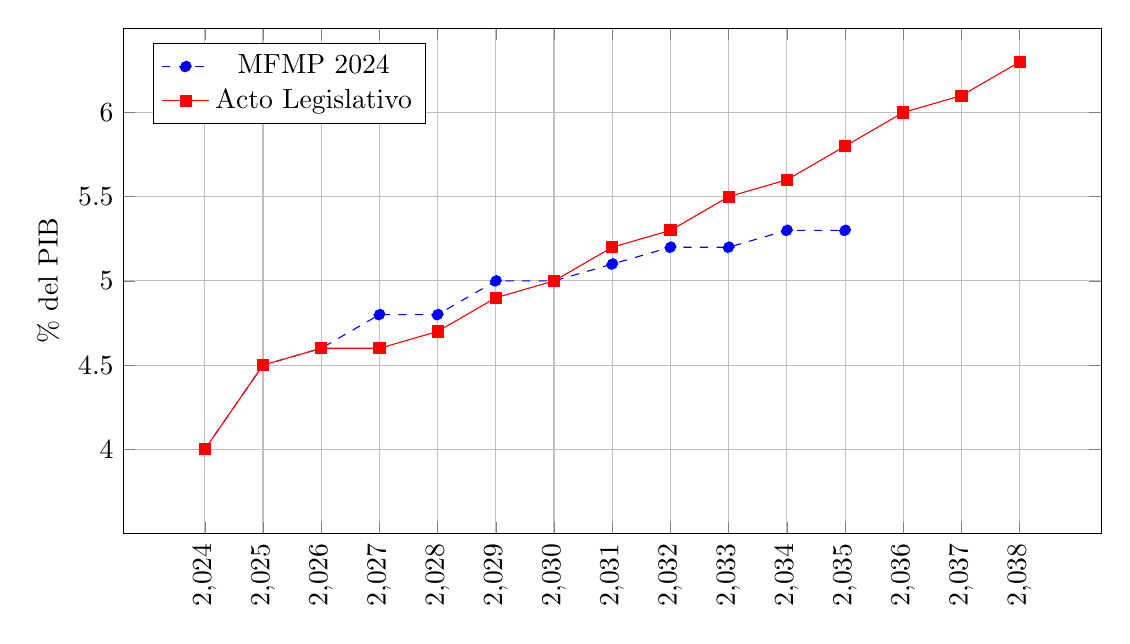
\begin{tikzpicture}
        \begin{axis}[
            width=14cm, height=8cm,
            ylabel={\% del PIB},
            xtick={%2023,
            2024,2025,2026,2027,2028,2029,2030,2031,2032,2033,2034,2035,2036,2037,2038},
            xticklabel style={rotate=90, anchor=east},
            ymin=3.5, ymax=6.5,
            legend pos=north west,
            grid=major,
            ytick={4,4.5,5,5.5,6},
        ]

        % MFMP 2024
        \addplot[color=blue, mark=*, dashed] coordinates {
            %(2023,3.4) 
            (2024,4.0) (2025,4.5) (2026,4.6) (2027,4.8)
            (2028,4.8) (2029,5.0) (2030,5.0) (2031,5.1) (2032,5.2)
            (2033,5.2) (2034,5.3) (2035,5.3)
        };
        \addlegendentry{MFMP 2024}

        % Acto Legislativo
        \addplot[color=red, mark=square*] coordinates {
            %(2023,3.4) 
            (2024,4.0) (2025,4.5) (2026,4.6) (2027,4.6)
            (2028,4.7) (2029,4.9) (2030,5.0) (2031,5.2) (2032,5.3)
            (2033,5.5) (2034,5.6) (2035,5.8) (2036,6.0) (2037,6.1) (2038,6.3)
        };
        \addlegendentry{Acto Legislativo}

        \end{axis}
    \end{tikzpicture}
    \vspace{0.1cm}
    \par\footnotesize{\textit{Fuente: Elaboración propia y MFMP 2024 del Ministerio de Hacienda.}}
\end{figure}


La Figura \ref{fig:sgp_forecast} muestra la proyección de las transferencias del \gls{gnc} al \gls{sgp} como porcentaje del PIB, bajo el nuevo escenario propiciado por el Acto Legislativo. Bajo este escenario, el \gls{sgp} presenta una tendencia creciente desde el 4,0\% del PIB en 2024 hasta el 6,3\% del PIB en 2038, un aumento de más de dos puntos del PIB. De nuevo se supone que los ingresos tributarios representan el 14,5\% del PIB en 2025, con un incremento anual de 0,1 puntos porcentuales debido a la gestión adicional de la \gls{dian}. Es clave resaltar este supuesto, ya que una reforma tributaria que aumente el recaudo llevaría a un aumento aún mayor de la participación del  \gls{sgp} sobre el PIB, superando la trayectoria prevista en la Figura \ref{fig:sgp_forecast}. Esto se debe a que el \gls{sgp} se define como un porcentaje de los ingresos corrientes de la Nación, los cuales provienen casi en su totalidad de los ingresos tributarios del \gls{gnc}. 

%\subsubsection{Ley de Competencias}
\subsection{Ley de Competencias}

A pesar de las dificultades inherentes al Acto Legislativo, la Ley de Competencias que lo regulará  brinda una oportunidad para contener algunos de sus efectos fiscales adversos. La Ley de Competencias es el instrumento que redefinirá las responsabilidades financieras entre el \gls{gnc} y las \gls{et}. Sin el traslado a las \gls{et} de responsabilidades financieras equivalentes, el incremento progresivo de las transferencias del \gls{sgp} generará una carga adicional sobre las finanzas públicas del \gls{gnc}, que se sumaría a las demás inflexibilidades de gasto. No obstante, esta carga desaparecerá si las \gls{et} asumen competencias adicionales en materia de formación técnica y tecnológica, educación superior, inversión pública, salud y primera infancia, como se a muestra a continuación.

\begin{table}[h!]
\centering
\caption{Costo de competencias del GNC transferibles a las ET (2024)}
\label{tab:costocomp}
\begin{tabular}{|l|c|}
\hline
\textbf{Competencia}            & \textbf{\% del PIB} \\
\hline
Inversión                   & 2,0 \\
Salud*                       & 2,4 \\
SENA e ICBF**                 & 0,2 \\
Universidades               & 0,4 \\
\hline
\textbf{Total}              & \textbf{5,0} \\
\hline
\end{tabular}
\vspace{0.1cm}
\par \footnotesize{*Incluye 4,4 de los 9 puntos porcentuales del impuesto a la renta del antiguo CREE}
\par \footnotesize{**Corresponde a 3,6 de los 9 puntos porcentuales del impuesto a la renta del antiguo CREE}
\par \footnotesize{\textit{Fuente: Elaboración propia con base en \cite{minhacienda_balance_2025}}}
\end{table}


La Tabla \ref{tab:costocomp} presenta el costo de algunas competencias actualmente a cargo del \gls{gnc} que podrían ser transferidas a las \gls{et}. Estas incluyen la inversión pública, la financiación de la salud, el \gls{sena}, el \gls{icbf} y las universidades públicas. En conjunto, dichas competencias representaron un gasto del 5,0\% del PIB en 2024. Esta cifra sirve como referencia para mostrar que el aumento proyectado de más de dos puntos del PIB en las transferencias del \gls{gnc} a las \gls{et} a través del \gls{sgp} puede ser fiscalmente viable, siempre que vaya acompañado de un traslado de las suficientes competencias.

En particular, se debería considerar que las \gls{et} concurran en la financiación del Servicio Nacional de Aprendizaje (\gls{sena}) y del Instituto Colombiano de Bienestar Familiar (\gls{icbf}), cuya participación conjunta por parte del \gls{gnc}  asciende a 0,2\% del PIB. De igual forma, las \gls{et} también podrían contribuir a la financiación de las universidades públicas, que representan otro 0,4\% del PIB. Asimismo, podrían aumentar su participación en la financiación del \gls{sgsss}, cuya financiación actual por parte del \gls{gnc} representa un 2,4\% del PIB. Finalmente, como se mencionó anteriormente en este capítulo, las \gls{et} también podrían asumir un rol más protagónico en materia de inversión pública, cuya financiación por parte del \gls{gnc} asciende al 2,0\% del PIB.

En el caso del \gls{sena} y el \gls{icbf}, se requerirá establecer sedes regionales con autonomía presupuestal y operativa, gestionadas directamente por los gobiernos distritales y departamentales. Las \gls{et} asumirían progresivamente una mayor proporción de los costos operativos y logísticos de los programas desarrollados por ambas instituciones. Eventualmente, cada sede regional contaría con plena autonomía operativa y financiera. Dicho esto, para viabilizar un traslado efectivo de competencias, sería necesario eliminar la destinación específica de los 3,6 puntos del impuesto de renta a las personas jurídicas que actualmente están asignados al \gls{sena} y al \gls{icbf}. Esta eliminación permitiría, por sí sola, reducir la tarifa general del impuesto de renta a las personas jurídicas del 35\% al 31,4\%, sin excluir la posibilidad de que cada \gls{et} establezca una sobretasa sobre dicho impuesto para financiar al \gls{sena} y al \gls{icbf}, como se argumenta más adelante. %Adicionalmente, la tarifa general del impuesto de renta a las personas jurídicas podría reducirse otro 4,4 puntos si la \gls{et} asumen la responsabilidad de financiar el sistema de salud en sus regiones, sin perjuicio de que puedan poner una sobretasa al impuesto de renta para financiar esta competencia tal como se discute más adelante.

Para las universidades públicas, sería necesaria la creación de un esquema de financiación en el cual las \gls{et} sean corresponsables de la financiación de las universidades públicas en su territorio. De hecho, el Acto Legislativo ya prevé que las \gls{et} concurran en la financiación de las universidades con lo equivalente a ``mínimo dos años del ciclo educativo de la educación superior''. Como es de esperarse, la Ley de Competencias deberá aclarar la forma en que se implementará esta concurrencia. Desafortunadamente, la concurrencia de recursos tanto nacionales como territoriales correría el riesgo de que el \gls{gnc} y las \gls{et} se acusen mutuamente de los incumplimientos financieros con las universidades, como ya ha pasado con el ejemplo de la Universidad de Antioquia.

Asimismo, la descentralización de la salud debe contemplar que las \gls{et} sean concurrentes en la responsabilidad de cubrir el déficit financiero del sistema de salud regional. Operativamente, el \gls{gnc} determinaría el aporte que debería tener cada \gls{et} en función de sus características demográficas y retenerlo del giro al \gls{sgp} para transferirlo directamente al \gls{adres}. En contraprestación, las \gls{et} deberán tener acceso a toda la información del manejo financiero y operativo del \gls{adres} para velar que la atención en salud en los municipios, distritos y departamentos efectivamente tenga correspondencia con los aportes realizados. 

Adicionalmente, la tarifa general del impuesto de renta a las personas jurídicas podría reducirse en otros 4,4 puntos si las \gls{et} asumen plenamente la responsabilidad de financiar el sistema de salud en sus regiones, sin perjuicio de que puedan establecer una sobretasa sobre el impuesto a la renta para cubrir dicha competencia. Estos 4,4 puntos corresponden a otra renta de destinación especiífica, en este caso destinada a la financiación del \gls{sgsss}.

La transferencia de competencias relacionada con la inversión pública también debe considerar incluir a las vigencias futuras para inversiones que han venido beneficiando a departamentos, distritos y municipios específicos. Como se discutió en el Capítulo \ref{chap:fepc}, las vigencias futuras representan una inflexibilidad adicional que limita la capacidad del \gls{gnc} para atender prioridades nacionales estratégicas y consolidar las finanzas públicas. Por tanto, es razonable que las \gls{et}, como beneficiarias directas de estos proyectos, asuman parte de su financiación en el marco del traslado de competencias.

Como complemento a la discusión sobre la inversión regional, es fundamental que el presupuesto de inversión de las \gls{et} se integre con el presupuesto del Sistema General de Regalías (\gls{sgr}), permitiendo una visión más coherente y coordinada de las necesidades de desarrollo regional. Esta articulación favorecerá una planeación más efectiva y reducirá la duplicidad en el uso de los recursos. En todo caso, tampoco debería descartarse la posibilidad de recentralizar el manejo del \gls{sgr} como contraprestación por el aumento en las transferencias del \gls{sgp}.

A pesar de estas medidas, persisten serias dudas sobre la capacidad de la mayoría de las \gls{et} para gestionar eficazmente el incremento en los recursos del \gls{sgp}, lo que pone en entredicho su potencial para cerrar las brechas regionales. La limitada capacidad administrativa y técnica de muchas de las \gls{et} podría traducirse en una ejecución ineficiente, desaprovechando la oportunidad de reducir las desigualdades sociales entre regiones. Por ello, es necesario que el \gls{gnc} fortalezca la supervisión de la gestión financiera subnacional y, cuando sea necesario, intervenga en la administración de las finanzas de las \gls{et} que incumplan los indicadores de gestión establecidos por la ley.

%\subsubsection{Sobretasas locales de IVA y renta}
\subsection{Sobretasas locales de IVA y de impuesto a la renta}

El Acto Legislativo establece que no se podrán descentralizar competencias sin la previa asignación de los recursos fiscales suficientes para atenderlas, y no se podrán asignar recursos a las \gls{et} sin la previa descentralización de competencias. Sin embargo, no toda transferencia de recursos debe canalizarse a través del \gls{sgp}. También es posible avanzar en la descentralización fiscal mediante el fortalecimiento de la autonomía tributaria territorial, dotando a las \gls{et} —particularmente a distritos y departamentos— de la capacidad para establecer sobretasas sobre el IVA y sobre el impuesto a la renta.

En este marco, se debe considerar impulsar una reforma tributaria que reduzca las tarifas generales de estos tributos a nivel nacional —como se discute en el Capítulo \ref{chap:masingresos}—, pero que al mismo tiempo habilite a distritos y departamentos para establecer sobretasas adicionales sobre dichos impuestos, aplicables exclusivamente en sus respectivas jurisdicciones. Por ejemplo, la tarifa general del impuesto de renta a las personas jurídicas podría reducirse del 35\% al 30\%, mientras que un departamento o distrito podría definir una sobretasa de 5 puntos porcentuales, de modo que la tarifa efectiva en esa región vuelva a ser del 35\%, con la diferencia asignada directamente a la respectiva \gls{et}. De manera análoga, la tarifa general del IVA podría disminuirse del 19\% al 16\%, permitiendo que distritos y departamentos establezcan su propia sobretasa, recaudada conjuntamente con el IVA nacional y transferida íntegramente a la \gls{et} que la adopte.

La aplicación de una sobretasa territorial sobre el IVA permitiría, además, viabilizar la eliminación del Impuesto de Industria y Comercio (ICA), en línea con la recomendación de la Comisión de Estudio del Sistema Tributario Territorial (\cite{CEDE2020}), que identificó este gravamen como una fuente de distorsiones significativas para la actividad económica local.

El recaudo generado por estas sobretasas sería transferido directamente a las \gls{et} que decidan implementarlas, sin pasar por el presupuesto del \gls{gnc}. De esta forma, las \gls{et} podrían financiar competencias que excedan aquellas cubiertas por el incremento del \gls{sgp}, en plena coherencia con el principio de equivalencia entre recursos y responsabilidades. Al mismo tiempo, el \gls{gnc} aliviaría sus presiones fiscales al trasladar a las \gls{et} competencias cuya financiación dependería de los propios gobiernos subnacionales, para lo cual se les otorgarían facultades en materia del IVA y del impuesto a la renta. Como se mencionó anteriormente, estas competencias podrían incluir la educación superior, la formación técnica y tecnológica, la atención integral a la primera infancia, el sistema de salud y la inversión pública. Dependerá de cada \gls{et} decidir las sobretasas, buscar fuentes de financiación complementarias y asumir las responsabilidades políticas de no recaudar lo suficiente para financiar sus nuevas responsabilidades.

No obstante, será necesario calibrar cuidadosamente la reducción en las tarifas generales con la selección de competencias a transferir, de manera que cada entidad territorial pueda decidir si impone las sobretasas y asume la financiación de las nuevas competencias, o si opta por no imponerlas y, en consecuencia, limita la ejecución de dichas responsabilidades. Esta flexibilidad permitiría adaptar el proceso de descentralización a las capacidades y prioridades de cada territorio.

Dicho lo anterior, es evidente que no todos los territorios tienen la misma capacidad económica para ejercer esta autonomía fiscal. Muchos municipios y departamentos carecen de una base productiva suficiente que les permita financiar con sobretasas las nuevas competencias. Por esta razón, resulta indispensable la creación de un fondo de compensación, el cual serviría para apoyar a las \gls{et} con menor capacidad fiscal (\cite{MisionDescentralizacionFECET}). Este fondo no debería financiarse con recursos provenientes de las sobretasas, sino con el aumento programado en la participación del \gls{sgp} dentro de los ingresos corrientes de la Nación, lo cual debe ser regulado en el marco de la Ley de Competencias.

%No obstante, será necesario calibrar cuidadosamente la reducción en las tarifas generales con la selección de competencias a transferir, de manera que cada entidad territorial pueda decidir si impone las sobretasas y asume la financiación de las nuevas competencias, o si opta por no imponerlas y, en consecuencia, limita la ejecución de dichas responsabilidades. Esta flexibilidad permitiría adaptar el proceso de descentralización a las capacidades y prioridades de cada territorio.

%Esta propuesta ofrece ventajas adicionales desde el punto de vista de los incentivos para la formalización de la actividad económica a nivel regional. En el sistema actual, las \gls{et} no cuentan con incentivos adecuados para promover la formalización de sus economías, ya que combatir la informalidad implica costos institucionales y políticos que pueden desincentivar la inversión en aquellas regiones donde se ejerce un mayor control, mientras que el recaudo adicional en IVA y en impuesto a la renta generado por la formalización se centraliza y se redistribuye a través del \gls{sgp}. Como resultado, las \gls{et} asumen los costos de la formalización sin recibir un retorno equivalente en términos de ingresos tributarios. En contraste, con la facultad de establecer sobretasas sobre el IVA y el impuesto de renta, se alinearían mejor los incentivos fiscales, promoviendo una participación más activa de los gobiernos subnacionales en la lucha contra la informalidad, la evasión y la elusión.


%Por supuesto, la facultad para cobrar las sobretasas también debe estar acompañado del traslado de competencias, de manera que se evita la duplicdad de funciones entre el \gls{gnc} y las \gls{et}. Como se mostró en la Tabla \ref{tab:costocomp}, el \gls{gnc} puede trasnferir competnecias e materia de inversión publica, formación técnica y tecnológica, educación superior, atención a la primera infancia y salud que vayan más allá de las competencias transferidas por el aumento del \gls{sgp}, siempre y cuando se le da las \gls{et} la capacidad de cobrar estas sobretasas. 


\subsection{Fórmula del SGP}

Aunque la Ley de Competencias podría subsanar parcialmente los problemas generados por el Acto Legislativo que reformó el \gls{sgp}, resulta imperativo volver a discutir la propia fórmula que determina el volumen de recursos transferidos. El núcleo del problema radica en haber atado el \gls{sgp} a un porcentaje fijo de los ingresos corrientes de la Nación, lo que limita severamente la efectividad de las reformas tributarias para avanzar en la consolidación fiscal, como se argumenta a continuación.

Si el \gls{sgp} se mantiene definido como un porcentaje de los ingresos corrientes de la Nación, cualquier reforma tributaria diseñada para incrementar los ingresos con el fin de reducir un déficit fiscal enfrenta un desafío que dificultará enormemente la consolidación fiscal. Supóngase por ejemplo que se quiere cerrar un déficit de \$10 billones mediante una reforma tributaria. Si el 39,5\% de los ingresos corrientes de la Nación deben destinarse al \gls{sgp}, la reforma tributaria requeriría en realidad recaudar \$16,5 billones. Esto obedece a que por cada peso adicional recaudado, el 39,5\% eventualmente se destinará al \gls{sgp}, por lo cual \$6,5 billones de los \$16,5 billones tendrían que destinarse al \gls{sgp} y no a cubrir el déficit que se intenta cerrar. 

Como está formulado, el \gls{sgp} introduce una barrera significativa para la consolidación fiscal al reducir la eficacia de las reformas tributarias. En la medida en que la participación del \gls{sgp} vaya aumentando, se tendrán que iterar varias reformas tributarias para poder compensar la parte adicional del recaudo que eventualmente se destinará al \gls{sgp}. Esto imposibilitaría que el país se despegue de su tradición de hacer una reforma tributaria cada dos años, con las consecuencias que eso conlleva sobre la estabilidad jurídica, la inversión y el crecimiento.  

Existen dos alternativas para mitigar el riesgo que representa, para la consolidación fiscal, la definición del \gls{sgp} como un porcentaje de los ingresos corrientes de la Nación. La primera consiste en redefinir el \gls{sgp} como un porcentaje del PIB en lugar de atarlo a los ingresos corrientes. Sin embargo, esta opción implicaría una reforma constitucional, pues requeriría modificar nuevamente la fórmula a través de un nuevo Acto Legislativo. La segunda alternativa es que los ingresos adicionales derivados de las reformas tributarias orientadas a la consolidación fiscal no se clasifiquen como ingresos corrientes y en cambio se clasifiquen como rentas de destinación específica para el pago de intereses sobre la deuda. Si bien el artículo 359 de la Constitución prohíbe las rentas de destinación específica, establece una excepción expresa para aquellas destinadas al servicio de la deuda pública.

%Como alternativa, los recursos destinados al SGP deben ser reformulados para que se midan como un porcentaje del PIB y no como porcentaje de los ingresos corrientes de la Nación. En particular, es necesario volver al Acto Legislativo y \textit{redefinir} una trayectoria para el SGP de tal forma que para que 12 años después de la ley de competencia la participación del SGP en el PIB alcance el mismo nivel que que se tenía proyectado cuando se definió el SGP como el 39.5\% de los ingresos corrientes de la Nación. Esta redefinición no es inocua dado que, para una trayectoria del SGP definida como porcentaje del PIB, un aumento de la participación de los ingresos corrientes de la Nación en el PIB (lo cual es necesario para estabilizar las finanzas públicas) no se traduce en un aumento del SGP. De esta forma se evitaría que las reformas tributarias, necesarias para solucionar los problemas fiscales actuales, pierdan eventualmente su eficacia.

%En ultima instancia, de persistir una formulación tan nociva como el monto del SGP en función de los ingresos corrientes de la Nación, el pago de intereses debería descontarse de los ingresos corrientes de la Nación. Desafortunadamente, Colombia ha transitado a una nueva situación semipermanente donde el pago de intereses a aumentado su participación relativo a los ingresos corrientes de la Nación, restando espacio para que aumente la participación del SGP sobre los ingresos corrientes de la Nación.

Por último, vale la pena recordar que el costo de las competencias transferidas no puede superar a los recursos transferidos. Como tal, las medidas discutidas están diseñadas para contener la presión fiscal creada por el Acto Legislativo, no para realizar ajustes de gasto. Por lo tanto, aunque es indispensable contener su impacto fiscal, el \gls{sgp} no ofrece un espacio de recorte para la consolidación fiscal.


\section{Gasto de personal}
%\vspace{0.3cm}
%\textbf{Gasto de personal}
%\vspace{0.1cm}

Como se mencionó en el Capitulo \ref{chap:fepc}, la participación del gasto de personal del \gls{gnc} en el PIB ha permanecido estable, al menos entre 2019 y 2024. No obstante, la evolución reciente de lo presupuestado para cubrir el costo de la nómina sugiere un aumento significativo del gasto de personal para 2025, como se infiere de la Tabla \ref{tab:nomina}. La tabla presenta el número de cargos y el costo anual de la nómina como porcentaje del PIB para los años 2023, 2024 y 2025, de acuerdo a lo presentado en los anexos presidenciales del \gls{pgn} para los mismos años. 

\begin{table}[h!]
    \caption{Nómina Pública (2023-2025)}
    \label{tab:nomina}
    \centering
    \begin{tabular}{lccc}
        \hline
        \textbf{Sector} & \textbf{2023} & \textbf{2024} & \textbf{2025} \\
        \hline
        \multicolumn{4}{c}{\textbf{Número de Cargos (miles)}} \\
        \hline
        Rama Ejecutiva (1) & 86 & 97 & 98 \\
        Militares y Policía (2) & 498 & 496 & 511 \\
        Judicial, Legislativa y otros (3) & 80 & 84 & 88 \\
        \hline
        \textbf{Total PGN (1+2+3)} & \textbf{663} & \textbf{678} & \textbf{696} \\ \hline
        SGP Educación (4) & 353 & 356 & 362 \\ 
        SGP Salud (5) & 47 & 46 & 49 \\
        Universidades (6) & 59 & 59 & 55 \\ \hline
        \textbf{Total Transferencias (4+5+6)} & \textbf{459} & \textbf{461} & \textbf{467} \\ \hline
        \textbf{Gran Total} & \textbf{1122} & \textbf{1139} & \textbf{1163} \\
        \hline
        \multicolumn{4}{c}{\textbf{Costo para la Nación (\% PIB)}} \\
        \hline
        Rama Ejecutiva (1) & 0,4 & 0,9 & 0,6 \\
        Militares y Policía (2) & 1,4 & 1,4 & 1,5 \\
        Judicial, Legislativa y otros (3) & 0,8 & 1,0 & 1,0 \\
        \textbf{Total PGN (1+2+3)} & \textbf{2,6} & \textbf{3,4} & \textbf{3,1} \\
        \hline
        SGP Educación (4) & 1,8 & 1,9 & 2,1 \\ 
        SGP Salud (5) & 0,2 & 0,2 & 0,2 \\
        Universidades (6) & 0,3 & 0,3 & 0,3 \\
        \textbf{Total Transferencias (4+5+6)}  & \textbf{2,3} & \textbf{2,4} & \textbf{2,6} \\
        \hline
        \textbf{Gran Total} & \textbf{4,9} & \textbf{5,8} & \textbf{5,8} \\
        \hline
    \end{tabular}
\vspace{0.3cm}
\par\footnotesize{\textit{Fuente: Elaboración propia con base en Anexos Presidenciales del PGN 2023, 2024 y 2025.}}  
\end{table}


Tal como se discutió en el Capítulo \ref{chap:fepc}, la nómina se puede dividir en aquella financiada directamente a través del \gls{pgn} y aquella financiada indirectamente a través de transferencias. Dentro de la nómina financiada directamente por el \gls{pgn} se encuentran: 1) la Rama Ejecutiva, 2) Militares y Policías, y 3) la Rama Legislativa, La Rama Judicial, la Fiscalía y los Organismos Autónomos. Dentro de la nómina financiada indirectamente a través de transferencias se encuentran: 4) los maestros (financiados a través del \gls{sgp} destinado a la educación), 5) personal de salud (financiados a través del \gls{sgp} destinado a la salud), y 6) los profesores universitarios y el personal administrativo de las universidades (financiados a través de la transferencia del \gls{gnc} a las universidades). Dado que las tres últimas son nóminas financiadas a través de transferencias, sólo las tres primeras nóminas son las que se contabilizan como gasto de personal del \gls{gnc}.

Si se compara la apropiación presupuestal de 2025 para el gasto de personal financiado directamente por el \gls{pgn} con la correspondiente de 2023, se observa un preocupante incremento de medio punto porcentual del PIB. Este aumento representa un gasto recurrente adicional difícil de revertir. Presumiblemente, este aumento obedece a un proceso de formalización del empleo público, entendido como la sustitución de contratistas por prestación de servicios por funcionarios de planta. Desafortunadamente, esta política se está implementando en un momento fiscal particularmente adverso, lo que agrava las inflexibilidades de gasto. 

Para mitigar el impacto fiscal del aumento en la nómina formal es necesaria la reducción del rubro de adquisición de bienes y servicios, dentro del cual se encuentran incluidos los contratistas por prestación de servicios. Aunque la formalización laboral implica trasladar parte de estos contratistas a la planta, muchos contratos persisten y coexisten con los nuevos cargos, generando una duplicación de funciones y un aumento neto del gasto. Por tanto, una estrategia responsable de formalización debe ir acompañada de una depuración rigurosa de los contratos temporales que permita evitar la duplicidad de funciones. 

Así mismo, es necesario avanzar en la reducción o fusión de entidades con funciones redundantes o mandatos superpuestos, donde la dispersión institucional ha dificultado la focalización del gasto y la rendición de cuentas. Un caso emblemático es el del recién creado Ministerio de la Igualdad y la Equidad, cuyas competencias se superponen con las de entidades como el Departamento para la Prosperidad Social. También existen importantes traslapos entre organismos de control, como la Procuraduría General, cuyas funciones disciplinarias podrían ser asumidas por las oficinas de control interno de cada entidad. Por último, las corporaciones autónomas regionales (CAR) presentan grandes disparidades en desempeño y han sido objeto de múltiples cuestionamientos por su baja eficiencia, limitada rendición de cuentas y alto riesgo de captura política. 

Dicho esto, hay que reiterar que la consolidación fiscal no puede depender exclusivamente de estas medidas, pues está presupuestado que en 2025 el gasto de personal del \gls{gnc} represente 3,1 puntos del PIB, de los cuales 1,5 puntos corresponden a militares y policías. Esto evidencia que el margen de ajuste en este componente del gasto es limitado y que se requieren otras medidas para lograr la consolidación fiscal.

\section{Conclusión}

Cualquier esfuerzo por recortar el gasto o aumentar los impuestos requerirá mejoras significativas en la percepción de legitimidad del Estado. En este sentido, el combate a la corrupción no es solo un instrumento para aumentar la eficiencia del gasto, sino una condición política indispensable para viabilizar el ajuste fiscal. La percepción de que los recursos públicos están siendo desviados mediante prácticas clientelistas o a través de esquemas como los cupos indicativos compromete la disposición de la ciudadanía a aceptar recortes de gasto o incrementos de impuestos. Por lo tanto, avanzar en una agenda de ajuste fiscal exige, en paralelo, una política clara de transparencia y un rechazo firme a las presiones clientelistas y corruptas que el Gobierno enfrentará al momento de impulsar las iniciativas legislativas necesarias para llevar a cabo la consolidación fiscal.

Implementar el ajuste del gasto requerirá que el nuevo Gobierno cuente con un amplio capital político y con la habilidad de comunicar —y convencer— sobre los beneficios de largo plazo que traería el saneamiento de las finanzas públicas. No obstante, el ajuste del gasto difícilmente podrá superar los dos puntos del PIB. A esto debe sumarse el esfuerzo por contener el crecimiento de las principales inflexibilidades del gasto, como las transferencias del \gls{sgp}, las pensiones y la salud. Suponiendo que la nueva Ley de Competencias logre reducir el costo de las competencias asumidas por el \gls{gnc} en una magnitud equivalente al aumento de las transferencias al \gls{sgp}, las mayores presiones vendrían entonces del gasto en salud y pensiones. Aun así, al menos otros dos puntos de ajuste fiscal deberán buscarse por el lado de los ingresos, como se discute a continuación en el Capítulo \ref{chap:masingresos}.
